\documentclass[10pt]{beamer}

\usetheme{CambridgeUS}
\usepackage[english, russian]{babel}
\usepackage[utf8]{inputenc}
\usepackage{caption}
\usepackage{minted}
\usepackage{etoolbox}
\usepackage{multicol}
\AtBeginEnvironment{minted}{\singlespacing%
    \fontsize{10}{10}\selectfont}

\title[\href{https://goo.gl/NRgp8K}{https://goo.gl/NRgp8K} (Term 1)]{Поиск подстрок}
\author[Гусев Илья]{Гусев Илья}
\institute[МФТИ] 
{Московский физико-технический институт\\*}
\date{Москва, 2017}
\subject{Computer Science}

\begin{document}

\begin{frame}
  \titlepage
\end{frame}

\begin{frame}{Содержание}
\tableofcontents
\end{frame}

\section{Функции}

\subsection{Префикс-функция}
\begin{frame}[fragile]{Префикс-функция}
Префикс-функция - массив чисел $\pi$, где $\pi[i]$ - такая наибольшая длина k наибольшего суффиксаs $s[i-k+1\ldots i]$ подстроки $s[0 \ldots i]$, совпадающего с её префиксом $s[0\dots k]$, но не совпадающего со всей строкой s.


\[\pi[s, i] = \max_{k=0 \ldots i} \{k: (s[0\dots k] = s[i-k+1\ldots i]) \}\]


Пример: abcabcd
\begin{center}
\begin{tabular}{ |c|ccccccc| } 
 \hline
 s & a & b & c & a & b & c & d \\ 
  \hline
$\pi$ & 0 & 0 & 0 & 1 & 2 & 3 & 0 \\ 
 \hline
\end{tabular}
\end{center}
\end{frame}

\begin{frame}[fragile]{Вычисление префикс-функции}
Утверждения:
\begin{enumerate}
\item $\forall i \rightarrow \pi[i+1] \leqslant \pi[i] + 1$
\item $\forall i:s[i+1] = s[\pi[i]] \rightarrow \pi[i+1] = \pi[i] + 1$
\item $\forall i:s[i+1] \ne s[\pi[i]] \rightarrow \pi[i+1] \le \pi[i]$
\end{enumerate}
На картинке $k = \pi[i]$
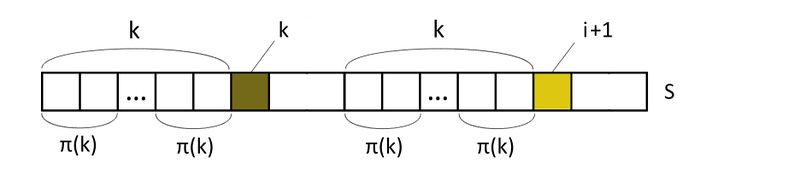
\includegraphics[width=13cm, height=3cm]{Term_3/Source/Pictures/prefix.jpg}


Для третьего случая итерируем $k = \pi[k]$, пока следующий символ не совпадёт.
\end{frame}

\begin{frame}[fragile]{Сложность вычисления префикс-функции}
\begin{multicols}{2}
Утверждения:
\begin{enumerate}
\item $\forall i \rightarrow \pi[i] < n-1$
\item $\pi$ по 1 разу за шаг вычисления, если выполняются условия 2 случая.
\item $\pi$ увеличивается не более, чем $n-1$ раз за весь алгоритм.
\item $\forall i \rightarrow \pi[i] \ge 0$
\item $\pi$ уменьшается не более, чем $n-1$ раз.
\item Всего не более $2\dot n$ шагов $\implies O(n)$
\end{enumerate}
\vfill\eject
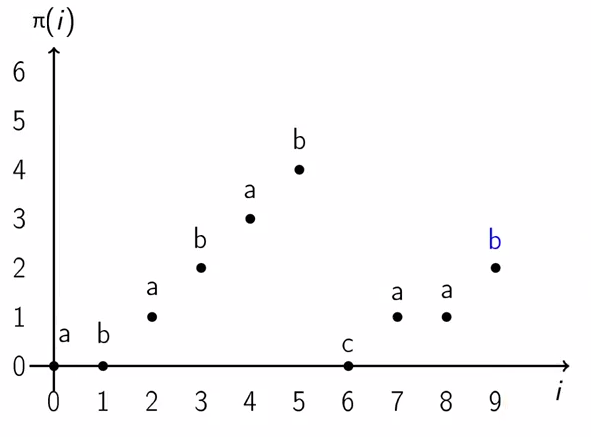
\includegraphics[width=6cm, height=4cm]{Term_3/Source/Pictures/prefix_graph.png}
\end{multicols}
\end{frame}


\begin{frame}[fragile]{Задача}
Найти \textbf{лексикографически-минимальную} строку, построенную по префикс-функции, в алфавите a-z.
Примеры: 
\begin{center}
\begin{tabular}{ |c|ccccccc| } 
 \hline
 $\pi$ & 0 & 0 & 0 & 1 & 2 & 3 & 0 \\ 
   \hline
 s & a & b & c & a & b & c & b \\ 
 \hline
\end{tabular}
\end{center}
\begin{center}
\begin{tabular}{ |c|cccccccc| } 
 \hline
 $\pi$ & 0 & 0 & 1 & 2 & 3 & 4 & 5 & 0 \\ 
   \hline
     s & a & b & a & b & a & b & a & c \\ 
 \hline
\end{tabular}
\end{center}
\end{frame}

\begin{frame}[fragile]{Решение}
\begin{enumerate}
    \item $\pi[i] \ne 0 \implies s[i] = s[\pi[i] - 1]$
    \item $\pi[i] = 0 \implies s[i] = \max \{s[\pi[i - 1]] + 1, s[\pi[\pi[i - 1]-1]]+1, \ldots] \}$\\
\end{enumerate}
Первое очевидно и следует напрямую из определения префикс-функции.\\
Второе опирается на несколько фактов:
\begin{enumerate}
    \item Нельзя допустить, чтобы новый символ сделал суффикс, совпадающий с  \textbf{каким-либо} префиксом по префиксам префиксов).
    \item +1 - всегда достаточно из-за того, что префикс всегда минимален. Делая +1 (например, из a в b) - гарантированно получаем 0 в префикс-функции.
    \item Из всех возможных вариантов продолжения выбираем минимальный.
\end{enumerate}
\end{frame}

\subsection{Z-функция}
\begin{frame}[fragile]{Z-функция}
Z-функция - массив чисел $z$, где $z[i]$ - длина наибольшего префикса строки s, который равен префиксу i-ого суффикса  $s[i \ldots n-1]$.

\[z[s, i] = \max_{k=0 \ldots n-1-i} \{k: (s[0\dots k] = s[i\ldots i+k]) \}\]


Примеры:
\begin{center}
\begin{tabular}{ |c|ccccc| } 
 \hline
 s & a & a & a & a & a\\ 
  \hline
z & 0 & 4 & 3 & 2 & 1 \\ 
 \hline
\end{tabular}
\end{center}
\begin{center}
\begin{tabular}{ |c|ccccccc| } 
 \hline
 s & a & a & a & b & a & a & b\\ 
  \hline
z & 0 & 2 & 1 & 0 & 2 & 1 & 0 \\ 
 \hline
\end{tabular}
\end{center}
\begin{center}
\begin{tabular}{ |c|ccccccc| } 
 \hline
 s & a & b & a & c & a & b & a\\ 
  \hline
z & 0 & 0 & 1 & 0 & 3 & 0 & 1 \\ 
 \hline
\end{tabular}
\end{center}
\end{frame}

\begin{frame}[fragile]{Задача}
Найти \textbf{лексикографически-минимальную} строку, построенную по z-функции, в алфавите a-z.
\begin{center}
\begin{tabular}{ |c|ccccc| } 
\hline
z & 5 & 3 & 2 & 1 & 0 \\ 
 \hline
 s & a & a & a & a & b\\ 
 \hline
\end{tabular}
\end{center}
\end{frame}

\begin{frame}[fragile]{Решение}
Один из возможных подходов:
\begin{enumerate}
\item z-функция $\implies$ префикс-функция
\item Решаем предыдущую задачу
\end{enumerate}
\end{frame}

\subsection{Z \rightarrow $\pi$}
\begin{frame}[fragile]{Z-функция $\implies$ префикс-функция}
Утверждения:
\begin{enumerate}
\item $\forall i \in [0, n), \forall j \in [0, z[i]) \rightarrow \pi[i+j] \ge j+1 $ 
\item $\forall i, \forall i', \forall j \in [0, z[i]), \forall j' \in [0, z[i']) :i < i', i+j = i'+j' \rightarrow \pi[i+j] = \pi[i'+j'] \ge j + 1 > j' + 1$ - на следующих итерациях значение префикс функции не увеличится
\item Если наталкиваемся на уже заданное значение $\pi$, переходим к $i+1$
\end{enumerate}
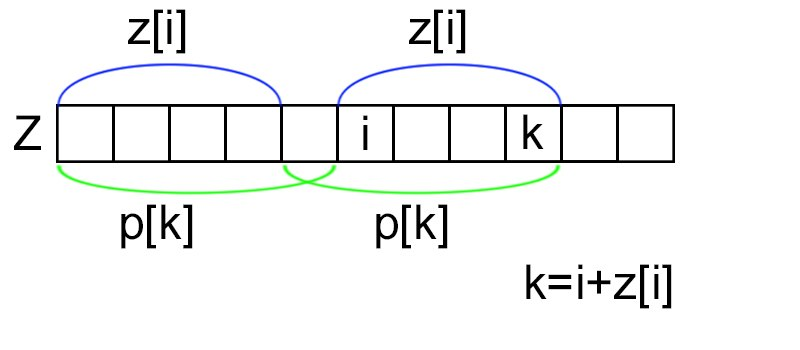
\includegraphics[width=7cm, height=3cm]{Term_3/Source/Pictures/z_to_p.jpg}\\

Сложность: $O(n)$, так как каждый элемент меняется ровно один раз и останавливаемся на каждом не более 1 раза.
\end{frame}

\section{Алгоритмы}
\subsection{Алгоритм Кнута—Морриса—Пратта}
\begin{frame}[fragile]{Алгоритм Кнута—Морриса—Пратта}
Дано: есть шаблон T, строка S, $len(T) < len(S)$.\\ 
Найти: все вхождения T в S.\\
Решение: $concat(T, \#, S)$, считаем префикс функцию. Где $\pi[i]=len(T)$, там и есть конец вхождения.\\
Сложность: $O(len(T) + len(S))$\\
Нюанс: при реализации запрещается хранить все значения префикс-функции! Ограничьтесь только нужными.
\end{frame}


\appendix
\section<presentation>*{\appendixname}
\subsection<presentation>*{Useful links}

\begin{frame}[allowframebreaks]
  \frametitle<presentation>{Полезные ссылки}
    
  \begin{thebibliography}{10}
{
  \beamertemplatebookbibitems
  % Start with overview books.


  \bibitem{Coursera01}
  \texttt{Видео про префикс-функцию на Курсере}
  \newblock \href{https://ru.coursera.org/learn/algorithms-on-strings/lecture/5lDsK/computing-prefix-function}{\texttt{https://ru.coursera.org/learn/algorithms-on-strings/lecture/\\5lDsK/computing-prefix-function}}
  
  \bibitem{emaxx1}
  \texttt{E-maxx: префикс-функция}
  \newblock \href{http://e-maxx.ru/algo/prefix_function}{\texttt{http://e-maxx.ru/algo/prefix\_function}}
  
  \bibitem{wiki}
  \texttt{Викиконспекты: префикс-функция}
  \newblock \href{https://neerc.ifmo.ru/wiki/index.php?title=\%D0\%9F\%D1\%80\%D0\%B5\%D1\%84\%D0\%B8\%D0\%BA\%D1\%81-\%D1\%84\%D1\%83\%D0\%BD\%D0\%BA\%D1\%86\%D0\%B8\%D1\%8F}{\texttt{https://neerc.ifmo.ru/wiki/index.php?title=Префикс-функция}}
  

  
  \bibitem{emaxx2}
  \texttt{E-maxx: z-функция}
  \newblock \href{http://e-maxx.ru/algo/z_function}{\texttt{http://e-maxx.ru/algo/z\_function}}
}
    
  \end{thebibliography}
\end{frame}

\end{document}


